% tikzpic.teP
\documentclass[crop,tikz]{standalone}% 'crop' is the default for v1.0, before it was 'preview'

%Packages
\usepackage{xcolor}

%tikz libraries}}
\usetikzlibrary{shapes.geometric}

%Colors
\definecolor{susceptible}{RGB}{141,160,203}
\definecolor{recovery}{RGB}{102,194,165}
\definecolor{infection}{RGB}{252,141,98}
\definecolor{intervention}{RGB}{50, 102, 86}
\definecolor{nothing}{RGB}{225,225,225}

% Formatting macros:
\tikzstyle{node}=[minimum size= .5in,circle, draw]
\tikzset{intervened node fill/.style  args={#1,#2}{node,circle split part fill={#1,#2}}}


\tikzstyle{edge}=[diamond, draw]
\tikzstyle{intervention}=[fill = intervention]
\tikzstyle{contact}=[fill = infection]
\tikzstyle{recovery}=[fill = recovery]

\makeatletter
\tikzset{circle split part fill/.style  args={#1,#2}{%
    alias=tmp@name, % Jake's idea !!
    postaction={%
      insert path={
        \pgfextra{%
          \pgfpointdiff{\pgfpointanchor{\pgf@node@name}{center}}%
          {\pgfpointanchor{\pgf@node@name}{north}}%
          \pgfmathsetmacro\scale{1}
          \pgfmathsetmacro\insiderad{\pgf@y*\scale}
          \fill[#1] (\pgf@node@name.base) ([yshift=-\pgflinewidth]\pgf@node@name.north) arc
          (90:270:\insiderad-\pgflinewidth)--cycle;
          \fill[#2] (\pgf@node@name.base) ([yshift=\pgflinewidth]\pgf@node@name.south)  arc
          (270:450:\insiderad-\pgflinewidth)--cycle;            %  \end{scope}
        }}}}}
 \makeatother  

\begin{document}


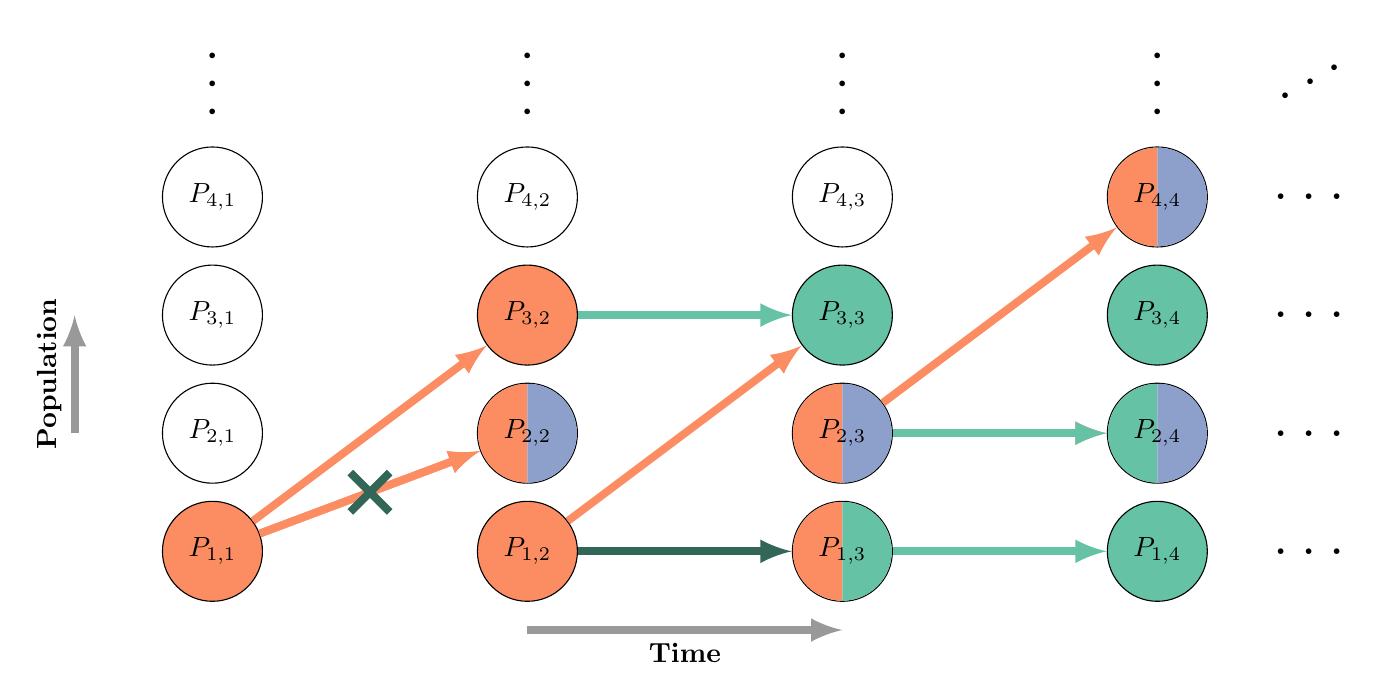
\begin{tikzpicture}
  \draw (0,0) node[node,contact] (P11) {$P_{1,1}$};
  \draw (0,1.5) node[node] (P21) {$P_{2,1}$};
  \draw (0,3) node[node] (P31) {$P_{3,1}$};
  \draw (0,4.5) node[node] (P41) {$P_{4,1}$};

  \draw (4,0) node[node,contact] (P12) {$P_{1,2}$};
  \draw (4,1.5) node[intervened node fill={infection,susceptible}] (P22) {$P_{2,2}$};
  \draw (4,3) node[node,contact] (P32) {$P_{3,2}$};
  \draw (4,4.5) node[node] (P42) {$P_{4,2}$};

  \draw (8,0) node[intervened node fill={infection,recovery}] (P13) {$P_{1,3}$};
  \draw (8,1.5) node[intervened node fill={infection,susceptible}] (P23) {$P_{2,3}$};
  \draw (8,3) node[node,recovery] (P33) {$P_{3,3}$};
  \draw (8,4.5) node[node] (P43) {$P_{4,3}$};

  \draw (12,0) node[node,recovery] (P14) {$P_{1,4}$};
  \draw (12,1.5) node[intervened node fill={recovery,susceptible}] (P24) {$P_{2,4}$};
  \draw (12,3) node[node,recovery] (P34) {$P_{3,4}$};
  \draw (12,4.5) node[intervened node fill={infection,susceptible}] (P44) {$P_{4,4}$};

  \draw[-latex,line width=1mm, color=infection] (P11) -- (P22);
  \draw[-latex,line width=1mm, color=infection] (P11) -- (P32);
  \draw[-latex,line width=1mm, color=infection] (P11) -- (P22);

  \draw[-latex,line width=1mm, color=infection] (P12) -- (P33);

  \draw[-latex,line width=1mm, color=infection] (P23) -- (P44);
  \draw[-latex,line width=1mm, color=infection] (P23) -- (P24);

  \draw[-latex,line width=1mm, color=intervention] (P12) -- (P13);
  \draw[-latex,line width=1mm, color=recovery] (P13) -- (P14);
  \draw[-latex,line width=1mm, color=recovery] (P32) -- (P33);
  \draw[-latex,line width=1mm, color=recovery] (P23) -- (P24);

  \draw[line width=1mm,color=intervention] (1.75,.5) -- (2.25,1);
  \draw[line width=1mm,color=intervention] (2.25,.5) -- (1.75,1);

  %% Extends on
  \draw (14,0) node{\Huge \dots};
  \draw (14,1.5) node{\Huge \dots};
  \draw (14,3) node{\Huge \dots};
  \draw (14,4.5) node{\Huge \dots};

  \draw (0,6) node[rotate=90]{\Huge \dots};
  \draw (4,6) node[rotate=90]{\Huge \dots};
  \draw (8,6) node[rotate=90]{\Huge \dots};
  \draw (12,6) node[rotate=90]{\Huge \dots};
  \draw (14,6) node[rotate=30]{\Huge \dots};
  %% Legend things
  \draw[-latex,line width=1mm,white!60!black] (4,-1) -- (8,-1) node[midway, below,text=black] {\textbf{Time}};
  \draw[-latex,line width=1mm,white!60!black] (-1.75,1.5) -- (-1.75,3) node[midway, above,text=black,rotate=90] {\textbf{Population}};
\end{tikzpicture}


\end{document}
